% C original page filename: codex/H134-06/pages/H134-06_134-2_scan182.tex
\scanpage{182}\mspage{37}%
% archive sheet number: 182
% L1a: raised parenthesis, with a long attachment guide entering after profinis.
les ``complétés profinis'' \inserted{(au sens d'Artin-Mazur)} premiers à $p$ (la car. de $k$) de tels espaces.
On voit clairement comment \unsure{aborder} un tel programme en car. $0$, mais on prévoit de l'amusement supplémentaire, voire du mystère, en car $p>0$, pour les variétés qui, même birationnellement, refuseraient de se laisser remonter en car. $0$!

% Separate rule: whole-image endpoints approximately (688,720) and (976,715).
\figure{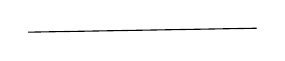
\begin{tikzpicture}
\draw[line width=0.4pt] (0,0) -- (2.9,0.05);
\end{tikzpicture}}

De ces cogitations essentiellement géométriques, je ne saurais à l'heure actuelle tirer un programme précis de développement de structures algébriques adéquates pour les exprimer.
Je me bornerai à quelques remarques en marge.

\deleted{\unsure{a|$\alpha$})} Depuis longtemps j'ai été \unsure{intrigu-|intrigué} par l'idée d'une ``linéarisation'' d'un type d'homotopie (ordinaire), i.e. la question du type: Si $X$ est un type d'homotopie, combien d'information cohomologique du type: cohomologie de $X$ à coefficients variables $M$ (constant%
% Compact detached point near (818,1807), below the first constant; physical presence retained, origin unassigned.
\raisebox{0pt}[0pt][0pt]{\parbox{0pt}{\figure{\begin{tikzpicture}[overlay,x=1pt,y=1pt]
\fill (-28,-7) circle[radius=0.35pt];
\end{tikzpicture}}}} ou constant tordus),
% A detached short vertical mark at approximately (271,1837), above the beginning of structure; origin uncertain.
\raisebox{2.2ex}[0pt][0pt]{\parbox{0pt}{\figure{\begin{tikzpicture}[overlay]
\draw[line width=0.3pt,line cap=round] (0.16,0) -- (0.17,-0.04) -- (0.17,-0.06) -- (0.18,-0.06);
\end{tikzpicture}}}}structure multiplicative
% The two short overwritten strokes favour = over +; the underlying sign remains doubtful.
% A distinct compact point at approximately (1024,1876), below the first H crossbar, is drawn without assigning it a mathematical role.
$\deleted{\unsure{=|+}}\raisebox{0pt}[0pt][0pt]{\parbox{0pt}{\figure{\begin{tikzpicture}[overlay]
\fill (0.09,0.05) ellipse [x radius=0.012cm,y radius=0.02cm];
\end{tikzpicture}}}}H^i(X,M)\times H^j(X,N)\mathrel{\unsure{\dashv|\to|-}}H^{\unsure{i\cdot j|i+j|ij}}(X,M\otimes N)$,
plus éventuellement d'autres opérations cohomologiques -- est-il%
% Detached short hooked stroke at approximately (1619,2077), well to the right of est-il; no word or punctuation function assigned.
\raisebox{0.4ex}[0pt][0pt]{\parbox{0pt}{\figure{\begin{tikzpicture}[overlay]
\draw[line width=0.3pt,line cap=round] (0.25,0) -- (0.27,-0.07) -- (0.31,-0.12);
\draw[line width=0.3pt,line cap=round] (0.27,-0.05) -- (0.26,-0.09);
\end{tikzpicture}}}} nécessaire d'avoir pour \unsure{réconstituer|rêconstituer} le type d'homotopie entièrement \deleted{\unsure{?}}? (disons,
